\begin{frame}
  \frametitle{Задача <<Змея в метро>>}
  \begin{center}
    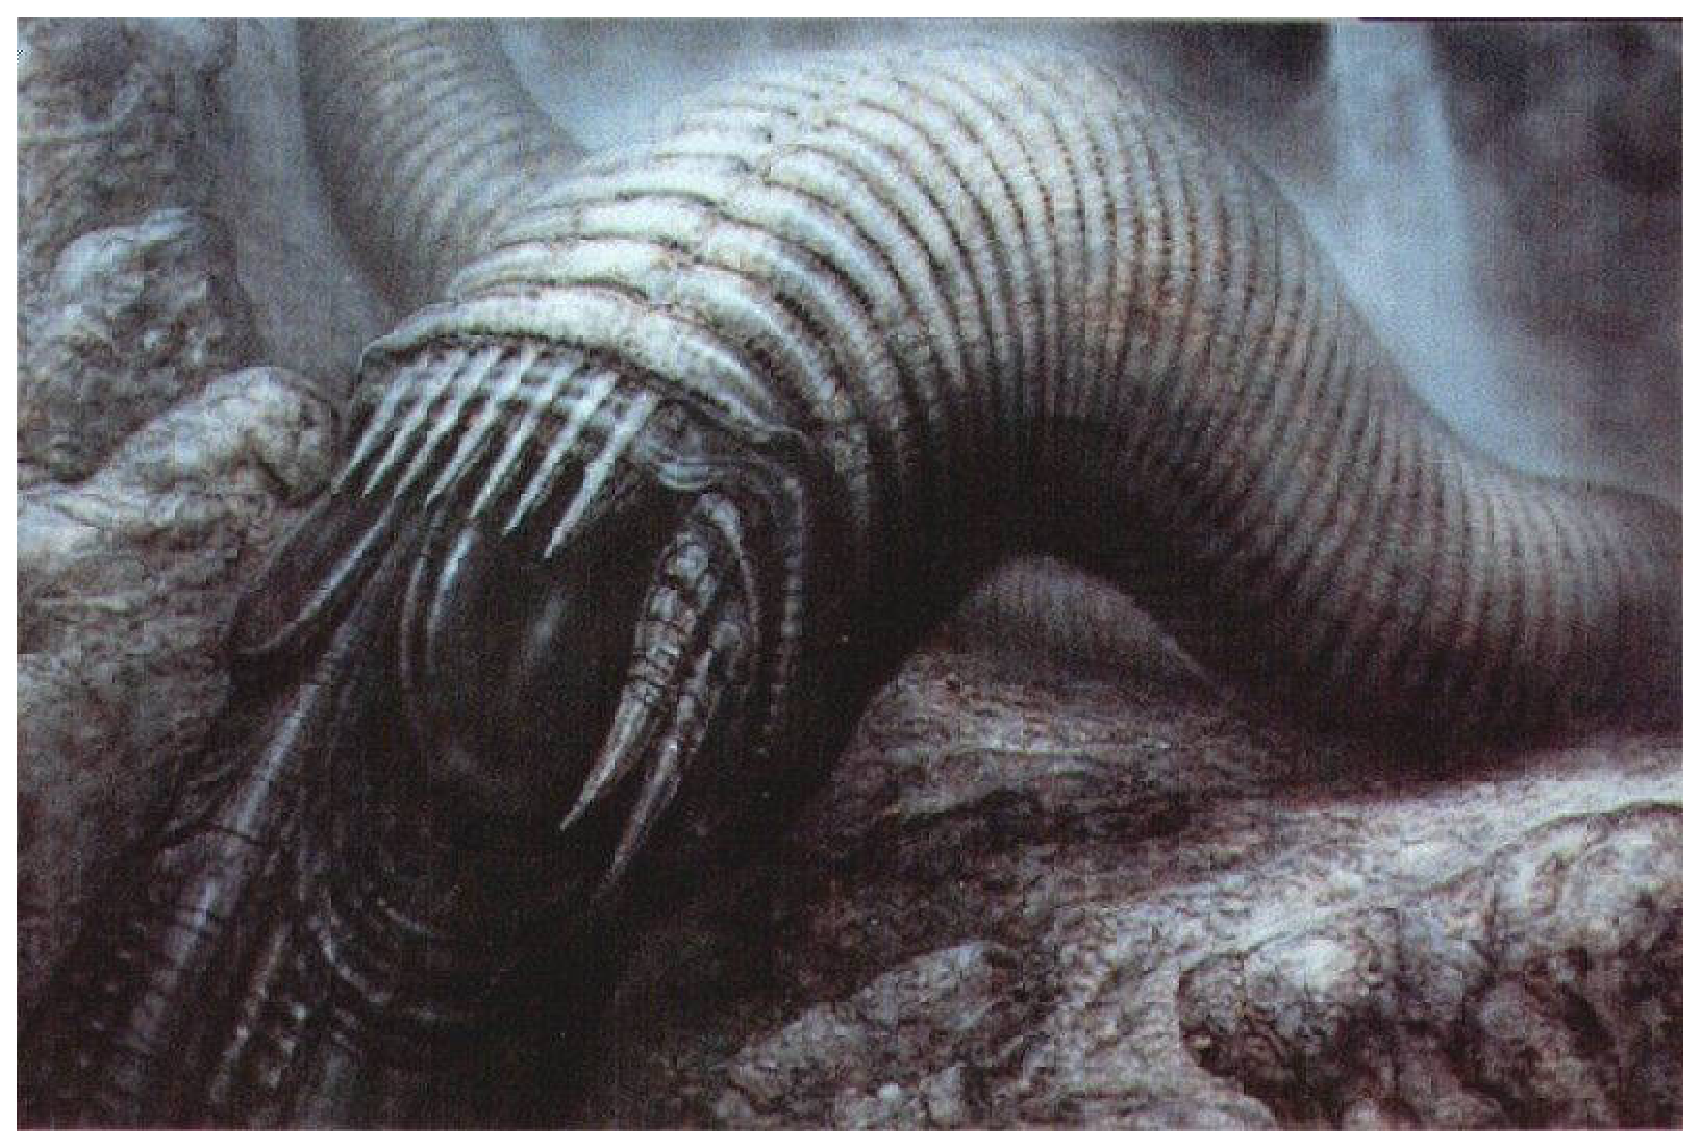
\includegraphics[width=10cm]{snake-11.eps}
  \end{center}
\end{frame}

\begin{frame}
  \frametitle{Над задачей работали}
  \begin{itemize}
    \item Идея задачи: Юрий Петров
    \item Текст условия: Юрий Петров
    \item Тесты, проверяющая программа и др.: Антон Ахи
    \item Решения: Антон Ахи, Антон Банных
    \item Текст разбора: Юрий Петров
  \end{itemize}
\end{frame}

\begin{frame}
  \frametitle{Формулировка задачи}
  \begin{itemize}
    \item Метро "--- граф
    \item Каждая вершина лежит не более, чем на одном простом цикле
    \item Змея лежит вдоль некоторого пути
    \item Змея не может самопересекаться
    \item Требуется найти кратчайший путь для змеи
  \end{itemize}
\end{frame}

\begin{frame}
  \frametitle{Идея решения}
  \begin{itemize}
    \item Заменим каждый цикл на вершину (например, с помощью обхода в глубину)
    \item Получится дерево
    \item Возможны два случая:
      \begin{itemize}
        \item Змея ориентирована в нужную сторону
        \item Змея ориентирована неправильно
      \end{itemize}
  \end{itemize}
\end{frame}

\begin{frame}
  \frametitle{Случай правильной ориентации}
  \begin{itemize}
    \item Требуется найти кратчайший путь любым обходом (в ширину, в глубину)
  \end{itemize}
\end{frame}

\begin{frame}
  \frametitle{Случай неправильной ориентации}
  \begin{itemize}
    \item Путь состоит из двух частей:
      \begin{itemize}
        \item Спуск вниз по дереву до цикла, где можно будет развернуться
        \item (развернуться можно, если длина цикла не меньше длины змеи)
        \item Подъём в обратную сторону
      \end{itemize}
  \end{itemize}
\end{frame}

\begin{frame}
  \frametitle{Итого}
  Вопросы?
\end{frame}
